\documentclass{standalone}
\usepackage{tikz}
\usetikzlibrary{patterns, positioning}
\usepackage[sfdefault]{ClearSans} %% option 'sfdefault' activates Clear Sans as the default text font
\usepackage[T1]{fontenc}

\begin{document}
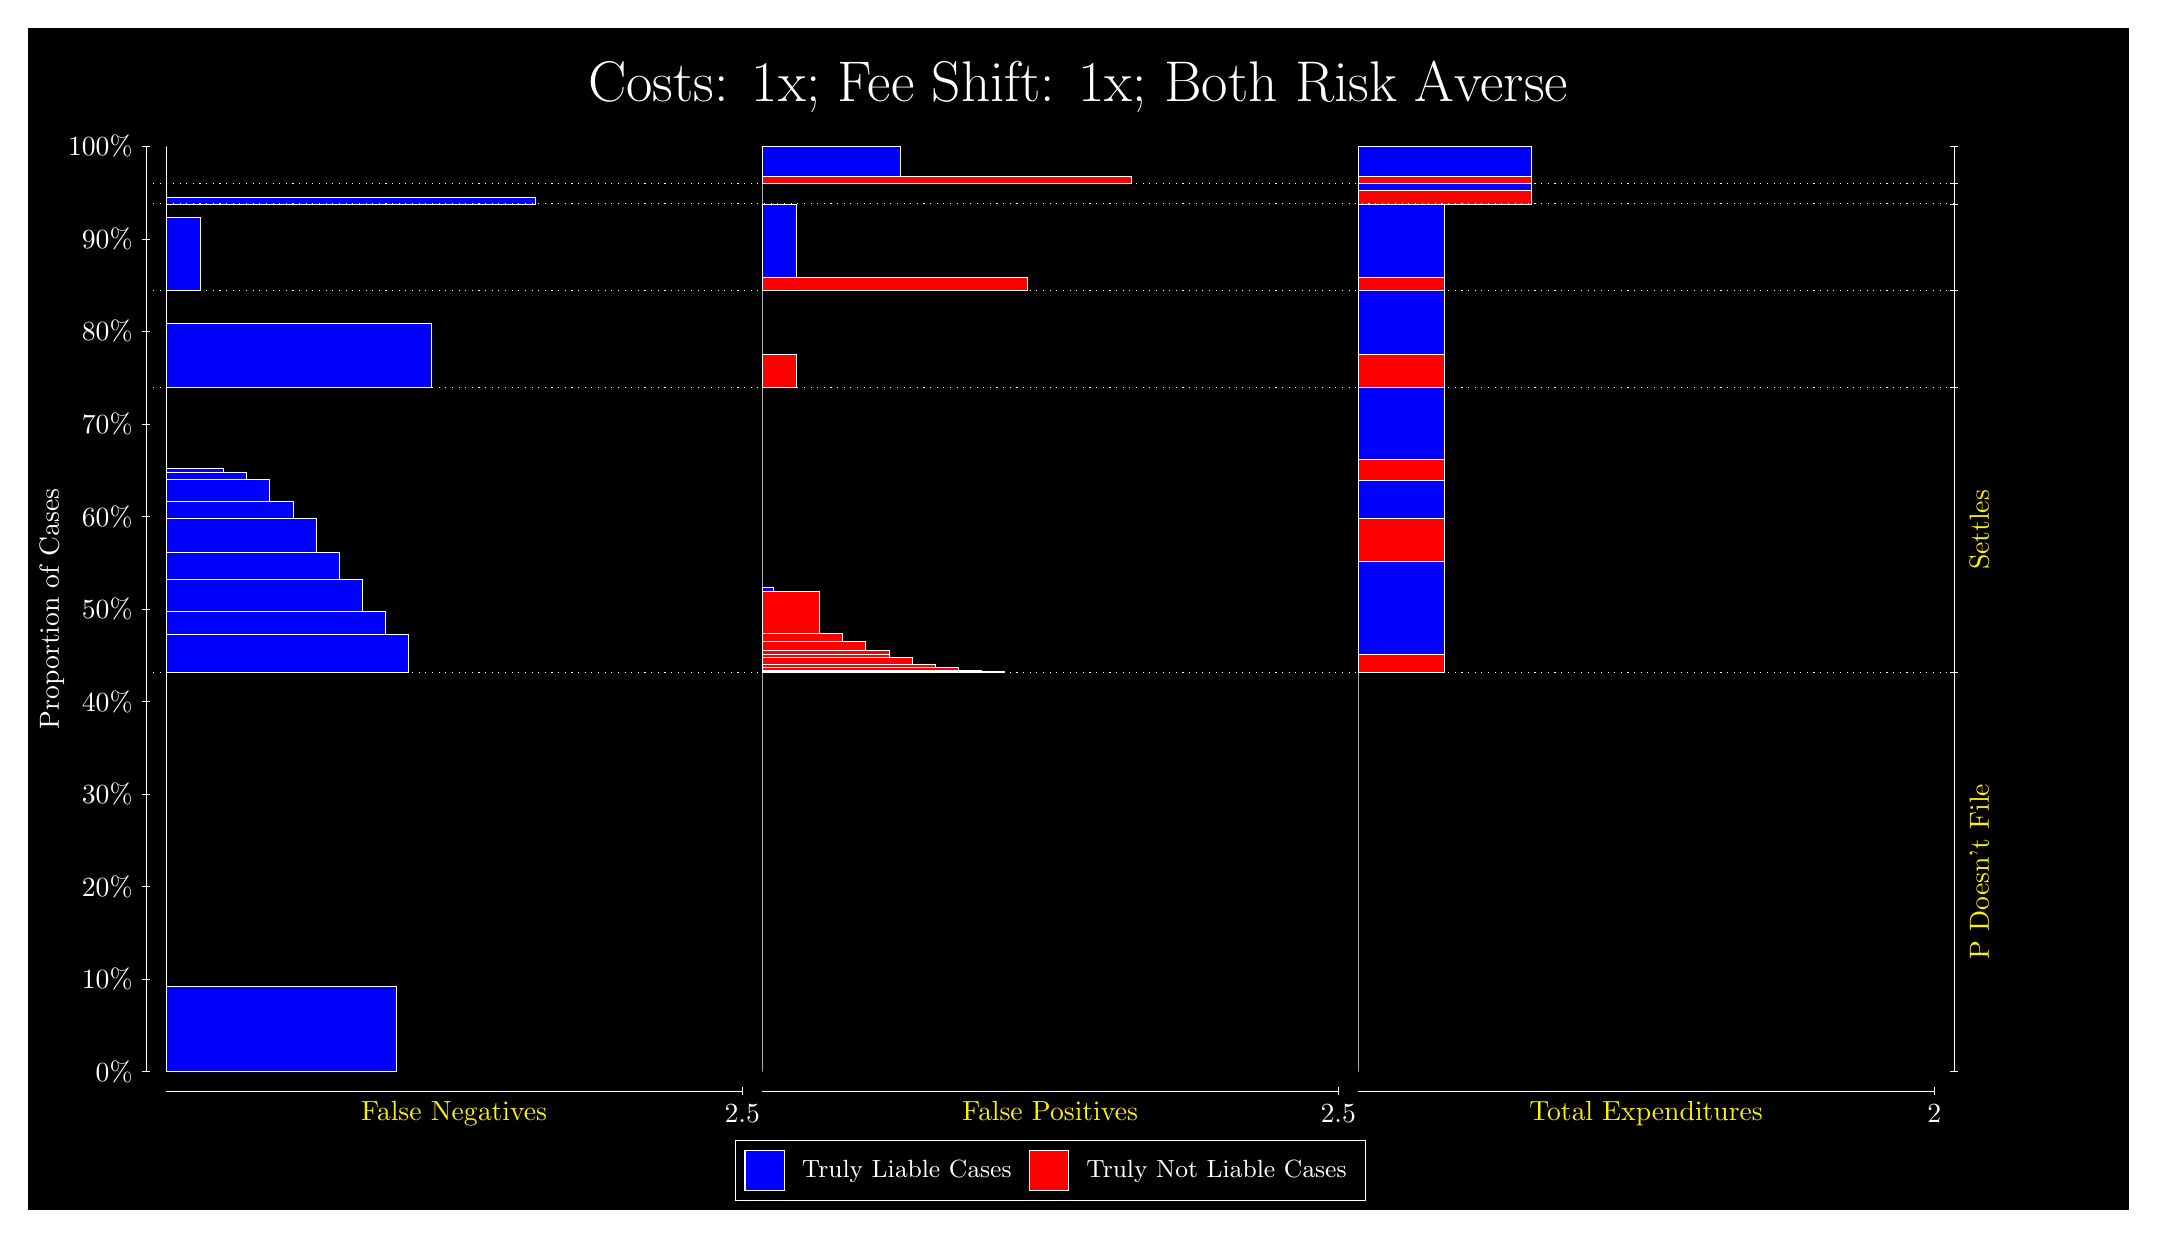
\begin{tikzpicture}
\draw[fill=black] (0,0) rectangle (26.667,15);
\draw[text=white] (0,13.5) rectangle (26.667,15) node[midway] {\huge Costs: 1x; Fee Shift: 1x; Both Risk Averse};
\draw[white, very thin] (1.5,1.75) -- (1.5,13.5);
\node[rotate=90, text=white, anchor=center] at (0.3, 7.625) {Proportion of Cases};
\draw[white, very thin] (1.45,1.75) -- (1.55,1.75);
\node[text=white, anchor=east] at (1.45, 1.75) {0\%};
\draw[white, very thin] (1.45,2.925) -- (1.55,2.925);
\node[text=white, anchor=east] at (1.45, 2.925) {10\%};
\draw[white, very thin] (1.45,4.1) -- (1.55,4.1);
\node[text=white, anchor=east] at (1.45, 4.1) {20\%};
\draw[white, very thin] (1.45,5.275) -- (1.55,5.275);
\node[text=white, anchor=east] at (1.45, 5.275) {30\%};
\draw[white, very thin] (1.45,6.45) -- (1.55,6.45);
\node[text=white, anchor=east] at (1.45, 6.45) {40\%};
\draw[white, very thin] (1.45,7.625) -- (1.55,7.625);
\node[text=white, anchor=east] at (1.45, 7.625) {50\%};
\draw[white, very thin] (1.45,8.8) -- (1.55,8.8);
\node[text=white, anchor=east] at (1.45, 8.8) {60\%};
\draw[white, very thin] (1.45,9.975) -- (1.55,9.975);
\node[text=white, anchor=east] at (1.45, 9.975) {70\%};
\draw[white, very thin] (1.45,11.15) -- (1.55,11.15);
\node[text=white, anchor=east] at (1.45, 11.15) {80\%};
\draw[white, very thin] (1.45,12.325) -- (1.55,12.325);
\node[text=white, anchor=east] at (1.45, 12.325) {90\%};
\draw[white, very thin] (1.45,13.5) -- (1.55,13.5);
\node[text=white, anchor=east] at (1.45, 13.5) {100\%};

\draw[white, very thin] (24.457,1.75) -- (24.457,13.5);
\draw[white, very thin] (24.407,1.75) -- (24.507,1.75);
\node[anchor=west] at (24.407, 1.75) {};
\draw[white, very thin] (24.407,6.822) -- (24.507,6.822);
\node[anchor=west] at (24.407, 6.822) {};
\draw[white, very thin] (24.407,10.435) -- (24.507,10.435);
\node[anchor=west] at (24.407, 10.435) {};
\draw[white, very thin] (24.407,11.668) -- (24.507,11.668);
\node[anchor=west] at (24.407, 11.668) {};
\draw[white, very thin] (24.407,12.769) -- (24.507,12.769);
\node[anchor=west] at (24.407, 12.769) {};
\draw[white, very thin] (24.407,13.031) -- (24.507,13.031);
\node[anchor=west] at (24.407, 13.031) {};
\draw[white, very thin] (24.407,13.5) -- (24.507,13.5);
\node[anchor=west] at (24.407, 13.5) {};

\draw[white, very thin, fill=blue] (1.75,1.75) rectangle (4.6775,2.8302);
\draw[white, very thin, fill=red] (1.75,2.8302) rectangle (1.75,6.822);
\draw[white, very thin, fill=blue] (1.75,6.822) rectangle (4.8239,7.3037);
\draw[white, very thin, fill=blue] (1.75,7.3037) rectangle (4.5312,7.597);
\draw[white, very thin, fill=blue] (1.75,7.597) rectangle (4.2384,8.0051);
\draw[white, very thin, fill=blue] (1.75,8.0051) rectangle (3.9457,8.3453);
\draw[white, very thin, fill=blue] (1.75,8.3453) rectangle (3.6529,8.77);
\draw[white, very thin, fill=blue] (1.75,8.77) rectangle (3.3602,8.9962);
\draw[white, very thin, fill=blue] (1.75,8.9962) rectangle (3.0674,9.2755);
\draw[white, very thin, fill=blue] (1.75,9.2755) rectangle (2.7746,9.3596);
\draw[white, very thin, fill=blue] (1.75,9.3596) rectangle (2.4819,9.4054);
\draw[white, very thin, fill=red] (1.75,9.4054) rectangle (1.75,10.435);
\draw[white, very thin, fill=blue] (1.75,10.435) rectangle (5.1167,11.248);
\draw[white, very thin, fill=red] (1.75,11.248) rectangle (1.75,11.668);
\draw[white, very thin, fill=blue] (1.75,11.668) rectangle (2.1891,12.598);
\draw[white, very thin, fill=red] (1.75,12.598) rectangle (1.75,12.769);
\draw[white, very thin, fill=blue] (1.75,12.769) rectangle (6.4341,12.853);
\draw[white, very thin, fill=red] (1.75,12.853) rectangle (1.75,13.031);
\draw[white, very thin, fill=red] (1.75,13.031) rectangle (1.75,13.117);
\draw[white, very thin, fill=blue] (1.75,13.117) rectangle (1.75,13.5);
\draw[white, very thin, fill=red] (9.3189,1.75) rectangle (9.3189,5.7418);
\draw[white, very thin, fill=blue] (9.3189,5.7418) rectangle (9.3189,6.822);
\draw[white, very thin, fill=red] (9.3189,6.822) rectangle (12.393,6.8308);
\draw[white, very thin, fill=red] (9.3189,6.8308) rectangle (12.1,6.8458);
\draw[white, very thin, fill=red] (9.3189,6.8458) rectangle (11.807,6.888);
\draw[white, very thin, fill=red] (9.3189,6.888) rectangle (11.515,6.9259);
\draw[white, very thin, fill=red] (9.3189,6.9259) rectangle (11.222,7.0134);
\draw[white, very thin, fill=red] (9.3189,7.0134) rectangle (10.929,7.0438);
\draw[white, very thin, fill=red] (9.3189,7.0438) rectangle (10.929,7.1012);
\draw[white, very thin, fill=red] (9.3189,7.1012) rectangle (10.636,7.2148);
\draw[white, very thin, fill=red] (9.3189,7.2148) rectangle (10.344,7.314);
\draw[white, very thin, fill=red] (9.3189,7.314) rectangle (10.051,7.8516);
\draw[white, very thin, fill=blue] (9.3189,7.8516) rectangle (9.4652,7.8974);
\draw[white, very thin, fill=blue] (9.3189,7.8974) rectangle (9.3189,10.435);
\draw[white, very thin, fill=red] (9.3189,10.435) rectangle (9.758,10.855);
\draw[white, very thin, fill=blue] (9.3189,10.855) rectangle (9.3189,11.668);
\draw[white, very thin, fill=red] (9.3189,11.668) rectangle (12.686,11.838);
\draw[white, very thin, fill=blue] (9.3189,11.838) rectangle (9.758,12.769);
\draw[white, very thin, fill=red] (9.3189,12.769) rectangle (9.3189,12.946);
\draw[white, very thin, fill=blue] (9.3189,12.946) rectangle (9.3189,13.031);
\draw[white, very thin, fill=red] (9.3189,13.031) rectangle (14.003,13.117);
\draw[white, very thin, fill=blue] (9.3189,13.117) rectangle (11.075,13.5);
\draw[white, very thin, fill=red] (16.888,1.75) rectangle (16.888,5.7418);
\draw[white, very thin, fill=blue] (16.888,5.7418) rectangle (16.888,6.822);
\draw[white, very thin, fill=red] (16.888,6.822) rectangle (17.986,7.0438);
\draw[white, very thin, fill=blue] (16.888,7.0438) rectangle (17.986,8.2359);
\draw[white, very thin, fill=red] (16.888,8.2359) rectangle (17.986,8.7735);
\draw[white, very thin, fill=blue] (16.888,8.7735) rectangle (17.986,9.2551);
\draw[white, very thin, fill=red] (16.888,9.2551) rectangle (17.986,9.5253);
\draw[white, very thin, fill=blue] (16.888,9.5253) rectangle (17.986,10.435);
\draw[white, very thin, fill=red] (16.888,10.435) rectangle (17.986,10.855);
\draw[white, very thin, fill=blue] (16.888,10.855) rectangle (17.986,11.668);
\draw[white, very thin, fill=red] (16.888,11.668) rectangle (17.986,11.838);
\draw[white, very thin, fill=blue] (16.888,11.838) rectangle (17.986,12.769);
\draw[white, very thin, fill=red] (16.888,12.769) rectangle (19.083,12.946);
\draw[white, very thin, fill=blue] (16.888,12.946) rectangle (19.083,13.031);
\draw[white, very thin, fill=red] (16.888,13.031) rectangle (19.083,13.117);
\draw[white, very thin, fill=blue] (16.888,13.117) rectangle (19.083,13.5);
\draw[white, dotted] (1.5,6.822) -- (24.457,6.822);
\draw[white, dotted] (1.5,10.435) -- (24.457,10.435);
\draw[white, dotted] (1.5,11.668) -- (24.457,11.668);
\draw[white, dotted] (1.5,12.769) -- (24.457,12.769);
\draw[white, dotted] (1.5,13.031) -- (24.457,13.031);
\draw[white, very thin] (1.75,1.5) -- (9.0689,1.5);
\node[text=yellow, anchor=north] at (5.4094, 1.5) {False Negatives};
\draw[white, very thin] (9.0689,1.45) -- (9.0689,1.55);
\node[text=white, anchor=north] at (9.0689, 1.45) {2.5};

\draw[white, very thin] (9.3189,1.5) -- (16.638,1.5);
\node[text=yellow, anchor=north] at (12.978, 1.5) {False Positives};
\draw[white, very thin] (16.638,1.45) -- (16.638,1.55);
\node[text=white, anchor=north] at (16.638, 1.45) {2.5};

\draw[white, very thin] (16.888,1.5) -- (24.207,1.5);
\node[text=yellow, anchor=north] at (20.547, 1.5) {Total Expenditures};
\draw[white, very thin] (24.207,1.45) -- (24.207,1.55);
\node[text=white, anchor=north] at (24.207, 1.45) {2};

\node[text=yellow, centered, rotate=90] at (24.777, 4.286) {P Doesn't File};
\node[text=yellow, centered, rotate=90] at (24.777, 8.6285) {Settles};





\draw (12.978300999999998,1.5) node[draw=none] (baseCoordinate) {};
\begin{scope}[align=center]
        \matrix[scale=0.5, draw=white, below=0.5cm of baseCoordinate, nodes={draw}, column sep=0.1cm]{
            \node[rectangle, draw, minimum width=0.5cm, minimum height=0.5cm, fill=blue] {}; &
            \node[draw=none, font=\small, text=white] (B) {Truly Liable Cases}; &
            \node[rectangle, draw, minimum width=0.5cm, minimum height=0.5cm, fill=red] {}; &
            \node[draw=none, font=\small, text=white] (B) {Truly Not Liable Cases}; \\
            };
\end{scope}

\end{tikzpicture}
\end{document}